\documentclass[10pt]{beamer}

\usepackage{multicol}
\usetheme[progressbar=frametitle]{metropolis}
\usepackage{appendixnumberbeamer}
\usepackage{anyfontsize}
\usepackage{booktabs}
\usepackage[scale=2]{ccicons}
\usepackage{pgfplots}
\usepgfplotslibrary{dateplot}
\usepackage{graphicx}
\usepackage{bussproofs}
\usepackage{xspace}
\usepackage{xcolor}
\newcommand{\themename}{\textbf{\textsc{metropolis}}\xspace}

\usepackage{listings}

\lstset
{ %Formatting for code in appendix
    language=C,
    numbers=left,
    stepnumber=1,
    basicstyle=\color{black}
}

%% https://github.com/nickgian/thesis/blob/master/lstcoq.sty
\usepackage{color}

\definecolor{ltblue}{rgb}{0,0.4,0.4}
\definecolor{dkblue}{rgb}{0,0.1,0.6}
\definecolor{dkgreen}{rgb}{0,0.35,0}
\definecolor{dkviolet}{rgb}{0.3,0,0.5}
\definecolor{dkred}{rgb}{0.5,0,0}

% lstlisting coq style (inspired from a file of Assia Mahboubi)
%
\lstdefinelanguage{Coq}{ 
%
% Anything betweeen $ becomes LaTeX math mode
mathescape=true,
%
% Comments may or not include Latex commands
texcl=false, 
%
% Vernacular commands
morekeywords=[1]{Section, Module, End, Require, Import, Export,
  Variable, Variables, Parameter, Parameters, Axiom, Hypothesis,
  Hypotheses, Notation, Local, Tactic, Reserved, Scope, Open, Close,
  Bind, Delimit, Definition, Let, Ltac, Fixpoint, CoFixpoint, Add,
  Morphism, Relation, Implicit, Arguments, Unset, Contextual,
  Strict, Prenex, Implicits, Inductive, CoInductive, Record,
  Structure, Canonical, Coercion, Context, Class, Global, Instance,
  Program, Infix, Theorem, Lemma, Corollary, Proposition, Fact,
  Remark, Example, Proof, Goal, Save, Qed, Defined, Hint, Resolve,
  Rewrite, View, Search, Show, Print, Printing, All, Eval, Check,
  Projections, inside, outside, Def},
%
% Gallina
morekeywords=[2]{forall, exists, exists2, fun, fix, cofix, struct,
  match, with, end, as, in, return, let, if, is, then, else, for, of,
  nosimpl, when},
%
% Sorts
morekeywords=[3]{Type, Prop, Set, true, false, option},
%
% Various tactics, some are std Coq subsumed by ssr, for the manual purpose
morekeywords=[4]{pose, set, move, case, elim, apply, clear, hnf,
  intro, intros, generalize, rename, pattern, after, destruct,
  induction, using, refine, inversion, injection, rewrite, setoid_rewrite, congr,
  unlock, compute, ring, field, fourier, replace, setoid_replace, fold, unfold,
  change, cutrewrite, simpl, have, suff, wlog, suffices, without,
  loss, nat_norm, assert, cut, trivial, revert, bool_congr, nat_congr,
  symmetry, transitivity, auto, split, left, right, autorewrite},
%
% Terminators
morekeywords=[5]{by, done, exact, reflexivity, tauto, romega, omega,
  assumption, solve, contradiction, discriminate},
%
% Control
morekeywords=[6]{do, last, first, try, idtac, repeat},
%
% Comments delimiters, we do turn this off for the manual
morecomment=[s]{(*}{*)},
%
% Spaces are not displayed as a special character
showstringspaces=false,
%
% String delimiters
morestring=[b]",
morestring=[d]’,
%
% Size of tabulations
tabsize=3,
%
% Enables ASCII chars 128 to 255
extendedchars=false,
%
% Case sensitivity
sensitive=true,
%
% Automatic breaking of long lines
breaklines=false,
%
% Default style fors listings
basicstyle=\small,
%
% Position of captions is bottom
captionpos=b,
%
% flexible columns
basewidth={2em, 0.5em},
columns=flexible,
%
% Style for (listings') identifiers
identifierstyle={\ttfamily\color{black}},
% Style for declaration keywords
keywordstyle=[1]{\ttfamily\bfseries\color{dkviolet}},
% Style for gallina keywords
keywordstyle=[2]{\ttfamily\bfseries\color{dkgreen}},
% Style for sorts keywords
keywordstyle=[3]{\ttfamily\bfseries\color{ltblue}},
% Style for tactics keywords
keywordstyle=[4]{\ttfamily\color{dkblue}},
% Style for terminators keywords
keywordstyle=[5]{\ttfamily\color{dkred}},
%Style for iterators
%keywordstyle=[6]{\ttfamily\color{dkpink}},
% Style for strings
stringstyle=\ttfamily,
% Style for comments
commentstyle={\ttfamily\itshape\color{dkgreen}},
%
%moredelim=**[is][\ttfamily\color{red}]{/&}{&/},
literate=
    {fun}{{\color{dkgreen}{$\lambda\;$}}}1
    {bool}{{$\mathbb{B}$}}1
    {nat}{{$\mathbb{N}$}}1
    {Vforall2}{Vforall2}1 % quick workardoun to avoid partial replacement of 'forall' in identifier
    {nat\_equiv}{nat\_equiv}1 % quick workardoun to avoid partial replacement of 'nat' in identifier
    {forall}{{\color{dkgreen}{$\forall\;$}}}1
    {exists}{{$\exists\;$}}1
    {<-}{{$\leftarrow\;\;$}}1
    {=>}{{$\Rightarrow\;\;$}}1
    {==}{{\texttt{==}\;}}1
    {==>}{{$\Longrightarrow\;\;$}}1
%    {:>}{{\texttt{:>}\;}}1
    {->}{{$\rightarrow\;\;$}}1
    {<-->}{{$\longleftrightarrow\;\;$}}1
    {<->}{{$\leftrightarrow\;\;$}}1
    {<==}{{$\leq\;\;$}}1
    {\#}{{$^\star$}}1 
    {\\o}{{$\circ\;$}}1 
%    {\@}{{$\cdot$}}1 
    {\/\\}{{$\wedge\;$}}1
    {\\\/}{{$\vee\;$}}1
    {++}{{\texttt{++}}}1
    {~}{{\ }}1
    {¬}{{$\lnot$}}1     % this does not work
    {\@\@}{{$@$}}1
    {\\mapsto}{{$\mapsto\;$}}1
    {\\hline}{{\rule{\linewidth}{0.5pt}}}1
%
}[keywords,comments,strings]

\lstnewenvironment{coq}{\lstset{language=Coq}}{}

% pour inliner dans le texte
\def\coqe{\lstinline[language=Coq, basicstyle=\small]}
% pour inliner dans les tableaux / displaymath...
\def\coqes{\lstinline[language=Coq, basicstyle=\scriptsize]}

%%% Local Variables: 
%%% mode: latex
%%% Local IspellDict: british
%%% TeX-master: "main.tex"
%%% End: 

\title{Formal Verification of Computer Programs}
\subtitle{A Primer. (part 2)}
% \date{\today}
\date{\date{}}
\author[shortname]{Vadim Zaliva \inst{1} \and Nika Pona \inst{2}}
\institute[shortinst]{\inst{1}Carnegie Mellon University \and \inst{2} Digamma.ai}

% \titlegraphic{\hfill\includegraphics[height=1.5cm]{logo.pdf}}

\begin{document}

\maketitle
\begin{frame}
\begin{abstract}

In this presentation we will introduce Coq's basic functionality and explain how Coq works internally.

\end{abstract}

\end{frame}

\begin{frame}{Table of contents}
  \setbeamertemplate{section in toc}[sections numbered]
  \tableofcontents[hideallsubsections]
\end{frame}



\section{Coq mini-intro}

\begin{frame}{Coq mini-intro}
  We did our proofs in a formal language called {\it Gallina}, a mechanized version of {\bf Calculus of Inductive Constructions}, which is a very expressive type theory well studied in mathematical logic. We write the specifications, model our programs and do the proofs in this language.

  \smallskip
We could do all of the above on paper, but it would quickly get out of hand. Moreover, we want to be sure that there are no mistakes in the proofs. So we use a tool called {\bf proof assistant}: a program that checks that your proof is correct. It also provides an environment to make the construction of proofs easier. 

In particular, we will talk about the Coq proof assistant: 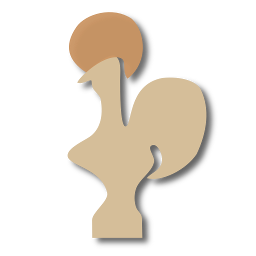
\includegraphics[width=1cm]{coq.png} \url{https://coq.inria.fr/}.

\end{frame}

\begin{frame}{What Coq does?}
  In Coq you can:
  \begin{itemize}
  
    \item define functions and predicates
    \item state mathematical theorems and software specifications
    \item interactively develop formal proofs of theorems
    \item machine-check these proofs by a relatively small trusted kernel
    \item extract certified programs to languages like OCaml, Haskell or Scheme.
  \end{itemize}
  
\end{frame}


\begin{frame}[fragile]{Inductive definitions}

  In Coq everything is either a {\it term} or a {\it type}. You can define basic inductive types using the \texttt{Inductive} command.

  \begin{lstlisting}[language=Coq]
  Inductive bool : Set :=
    | true : bool
    | false : bool.

  \end{lstlisting}

  The boolean type has two {\bf constructors}: \texttt{true} and \texttt{false}.  
  
   \begin{lstlisting}[language=Coq]
  Inductive nat : Set :=
    | O : nat
    | S : nat -> nat.  
   \end{lstlisting}

   Natural numbers are defined by two constructors as well: \texttt{O} (zero) and \texttt{S} (successor function). Any {\it term} of type $\mathbb{N}$ is constructed using these two. E.g., \texttt{S O} : $\mathbb{N}$, \texttt{S (S O)} : $\mathbb{N}$, \texttt{S (S (S O))} : $\mathbb{N}$  \ldots
\end{frame}

\begin{frame}[fragile]{Recursive definitions}

  You can define recursive functions using the \texttt{Fixpoint} command.

  Since we know that by construction any term of type $\mathbb{N}$ is either \texttt{O} or \texttt{S n} for some $n : \mathbb{N}$, we can use {\it pattern-matching}.
  
   \begin{lstlisting}[language=Coq]
  Fixpoint plus (n m : nat) : nat :=
  match n with
  | O => m
  | S p => S (plus p m)
  end
   \end{lstlisting}
   
Note: Coq only accepts definitions that terminate\footnote{This limitation is needed to ensure consistency of the system, as well as decidability of type-checking.}. Here we are recursing on a direct subterm of $n$ thus we are guaranteed to terminate and Coq is able to automatically ensure this. Sometimes you have to do a termination proof by hand. 
\end{frame}


\begin{frame}[fragile]{Proofs}


  Finally, you can state and prove theorems about the objects you defined. Let $+$ be notation for \texttt{plus}.

  \begin{theorem} 2 + 3 = 5.
    \end{theorem}

  How would you prove this, if you were to justify each step of the proof?
  
  \begin{lstlisting}[language=Coq]
Theorem plus_2_3 : (S (S O)) + (S (S (S O))) = (S (S (S (S (S O))))).
 Proof.
  unfold plus. (* apply definition of plus *)
  reflexivity. (* apply definition of equality *)
 Qed.

  \end{lstlisting}
  In Coq you constructs a proof using so-called {\sf tactics}.
  E.g., \texttt{simpl} is a tactic that performs basic application of definitions, \texttt{reflexivity} proves equality between two syntactically equal terms (modulo some reductions).  
 
\end{frame}


\begin{frame}{Demo}
\end{frame}

\begin{frame}<0>[fragile]{More proofs}
\begin{theorem} $\forall n,\ 0 + n = n$.
\end{theorem}

To prove this we also use the definition of addition: since the recursion is on the first term, we are in the base case.

   \begin{lstlisting}[language=Coq]
  Fixpoint plus (n m : nat) : nat :=
  match n with
  | O => m (* base case *)
  | S p => S (plus p m)
  end
   \end{lstlisting}

   Proof in Coq:

  \begin{lstlisting}[language=Coq]
    Theorem plus_O_n : (forall n, O + n = n).
    Proof.
      intros n. (* take any n *)
      simpl. (* apply definition of plus *)
      reflexivity. (* get equal terms *)
    Qed.
  \end{lstlisting}

 
\end{frame}



\begin{frame}<0>[fragile]{More proofs}

  Most proofs would need to go by induction (Why the previous proof won't work below? See how \texttt{plus} is defined.)

  \begin{lstlisting}[language=Coq]
    Theorem plus_n_O : (forall n, n + O = n).
    Proof.
      (* proof by induction on n *)
      induction n; simpl.
      (* base case *)
      - reflexivity.
      (* inductive step *)
      - rewrite IHn. (* apply induction hypothesis *)
        reflexivity.
    Qed.

  \end{lstlisting}
\end{frame}
\begin{frame}{More Proofs}
     In Coq you have to justify every step of the proof and the \texttt{Qed} command only succeeds on correct proofs. But you don't have to do every proof from scratch, since there are extensive libraries covering lemmas about basic mathematics as well as several decision procedures that automatize proof search.
     \begin{itemize}
     \item Using SMT and SAT solvers: \url{https://smtcoq.github.io/}
     \item First-order decision procedures (CoqHammer): \url{https://github.com/lukaszcz/coqhammer}
     \item Tactics for solving arithmetic goals over ordered rings (\texttt{Micromega})
       \item And much more, cf. \url{https://coq.inria.fr/opam/www/}
       \end{itemize}
  
\end{frame}

   \section{How does Coq work?}
\begin{frame}{How does Coq work?}
    We can formalize programs, properties and proofs in the same language, as well as efficiently and reliably check proof correctness due to the so-called {\bf Curry-Howard Isomorphism}.

    Curry-Howard isomorphism is a correspondence between programs and terms on one hand and proofs and types on the other. All logical statements in Coq are typing judgments and thus checking the correctness of proofs amounts to type checking. Let's see what it means precisely on a small example.
   \end{frame}
   
   \begin{frame}{Curry-Howard Isomorphism (CHI)}
     We said that {\it ``Curry-Howard Isomorphism is a correspondence between programs and terms on one hand and proofs and types on the other''}. To make this precise, we need to specify what kind of programs we have on one side and what kind of proofs (that is, what kind of logic) we have on the other side.

     Various {\bf lambda calculi} were designed to describe programs.% {\it untyped lambda-calculus, simply-typed lambda calculus, polymorphic lambda-calculus, G\"{o}del's system {\bf T}, system {\bf F}} etc\footnote{cf. Lectures on Curry-Howard Isomorphism \cite{Sørensen98lectureson}}.
     If you never heard of lambda calculi, think of functional programming languages such as {\bf LISP},  {\bf OCaml}, and {\bf Haskell}.
     
\end{frame}
\begin{frame}{The untyped lambda calculus}
    Consider the simplest example of lambda calculus\footnote{Or a rudimentary functional programming language.}: the untyped lambda calculus. The terms are:
     \begin{description}
     \item[Var] variables
     \item[Abs] $(\lambda x.M)$, if $x$ a variable and $M$ is a term 
     \item[App] $(M N)$, if $M$ and $N$ are terms
     \end{description}
     Think of $(\lambda x.M)$ as a function with argument $x$ and body $M$ and of $(M N)$ as applying function $M$ to the argument $N$\footnote{For more details see \cite{Sørensen98lectureson}.}. %This is formalized by introducing $\beta$-{\it reduction} relation on terms:
     %\[ (\lambda x.M)N \Rightarrow_\beta M[x := N]\footnote{Meaning substitute all occurences of x in M by N.} \] 
%Some examples of $\beta$-reduction: 
 %    \[ (\lambda x.x)y \Rightarrow_\beta y \]
  %   \[ ((\lambda x.(x z)) y \Rightarrow_\beta (y z) \]

\end{frame}

\begin{frame}{The untyped lambda calculus (cont.)}
       
     In lambda calculus one could encode basic constructs such as natural numbers and lists, as well as functions on them and logical constants and operations. Using the \textit{Y combinator} recursive functions could be encoded as well.

     Examples of terms:

     $id = \lambda x.x$ (identity function)
     
\end{frame}

\begin{frame}[fragile]{Church Booleans}
       
    We can encode boolean algebra using our calculus.
    
    The \emph{True} and \emph{False} values:
\begin{align*}
\mathrm{true} &= \lambda t.\lambda f. t \\
\mathrm{false} &= \lambda t.\lambda f. f
\end{align*}

    And some basic boolean algebra operations:   
\begin{align*}
\mathrm{and} &= \lambda b. \lambda c. (b\ c\ \mathrm{false}) \\
\mathrm{or}  &= \lambda x. \lambda y. (x\ \mathrm{true}\ (y\ \mathrm{true}\ \mathrm{false})) \\
\mathrm{not} &= \lambda b. (b\ \mathrm{false}\ \mathrm{true})
\end{align*}

\end{frame}

\begin{frame}{Church Numerals}
    Similarly, we can encode \textit{natural numbers}:
\begin{align*}
c_0 &= \lambda s.\lambda z. z \\
c_1 &= \lambda s.\lambda z. s z \\
c_2 &= \lambda s.\lambda z. s (s z) \\ 
c_3 &= \lambda s.\lambda z. s (s (s z)) \\
\text{\textit{etc.}}
\end{align*}

    And some basic arithmetic operations:   
\begin{align*}
\mathrm{succ} &= \lambda n. \lambda s. \lambda z.\ s\ (n\ s\ z)\\
\mathrm{plus} &= \lambda m. \lambda n. \lambda s. \lambda z.\ m\ s\ (n\ s\ z)\\
\mathrm{times} &= \lambda m. \lambda n.\ m\ (\mathrm{plus}\ n)\ c_0
\end{align*}

\end{frame}

\begin{frame}{Simply typed lambda-calculus}
       We are interested in a {\bf typed} lambda calculus. The types of {\bf ST} are:
        \begin{description}
     \item[Var] type variables 
     \item[Arrow] $\tau \rightarrow \sigma$, if $\tau$ and $\sigma$ are types
       \end{description}
       Types are assigned to terms according to certain rules. Let $\Gamma$ be a set of simply-typed terms (also called context). 
       \begin{prooftree}
          \AxiomC{$\Gamma, x : \tau \vdash x : \tau $ ({\bf Ax})}     
                 \end{prooftree}

         \begin{prooftree}
           \AxiomC{$\Gamma, x : \sigma \vdash M : \tau$}
           \RightLabel{({\bf Abs})}
           \UnaryInfC{$\Gamma \vdash (\lambda x. M) : \sigma \rightarrow \tau$}
         \end{prooftree}

         \begin{prooftree}
           \AxiomC{$\Gamma \vdash M : \sigma \rightarrow \tau$}
           \AxiomC{$\Gamma \vdash N : \sigma$}
           \RightLabel{({\bf App})}
           \BinaryInfC{$\Gamma \vdash (M N) : \tau$}
         \end{prooftree}
\end{frame}
\begin{frame}{Type derivation}
         Here is a simple derivation that shows that the term $\lambda x. x$ (identity) has type $\sigma \rightarrow \sigma$, with $\sigma$ being any type of {\bf ST}: \begin{prooftree}
          \AxiomC{$ x : \sigma \vdash x : \sigma$ ({\bf Ax})}
          \RightLabel{({\bf Abs})}
           \UnaryInfC{$\vdash (\lambda x. x) : \sigma \rightarrow \sigma$}
         \end{prooftree}

And if you apply identity to a term of type $\sigma$, the output is also of type $\sigma$:

\begin{prooftree}
          \AxiomC{$ y : \sigma, x : \sigma \vdash x : \sigma$ ({\bf Ax})}
          \RightLabel{({\bf Abs})}
           \UnaryInfC{$y : \sigma, \vdash (\lambda x. x) : \sigma \rightarrow \sigma$}
           \AxiomC{ $y : \sigma \vdash y : \sigma$ ({\bf Ax})}
           \RightLabel{({\bf App})}
           \BinaryInfC{ $y : \sigma \vdash ((\lambda x. x) y) : \sigma$}
         \end{prooftree}
         \end{frame}
         
\begin{frame}<0>
A more complex example.         
          \begin{prooftree}
            \AxiomC{$y : \tau, x : \tau \rightarrow \sigma \vdash x : \tau \rightarrow\sigma$ ({\bf Ax})}
            \AxiomC{$y : \tau, x : \tau \rightarrow \sigma \vdash y : \tau$ ({\bf Ax}) }
          \RightLabel{({\bf App})}
          \BinaryInfC{$y : \tau, x : \tau \rightarrow \sigma  \vdash (x y) : \sigma$}
          \RightLabel{({\bf Abs})}
          \UnaryInfC{$ y : \tau \vdash \lambda x. (x y) : (\tau \rightarrow \sigma) \rightarrow \sigma$}
          \RightLabel{({\bf Abs})}
          \UnaryInfC{$\vdash \lambda y.\lambda x. (x y) : \tau \rightarrow (\tau \rightarrow \sigma) \rightarrow \sigma$}
         \end{prooftree}
\end{frame}
\begin{frame}{Back to CHI}
         We made one side of the Curry-Howard Correspondence more precise: the simply typed lambda calculus, which corresponds to some rudimenatry functional programming language. Now: what does it correspond to and how?

         In general programs (or computations) will correspond to certain kind of logics. Namely, {\bf intuitionistic logics}. These logics were created to formalize what is called constructive mathematics: that is, mathematics in which we are only interested in objects that can be effectively constructed.
\end{frame}
   
\begin{frame}{Implicational propositional logic}
     Consider the simplest intuitionistic logic {\bf Impl}. The formulae of {\bf Impl} are the following: 
     \begin{description}
     \item[Var] propositional variables 
     \item[Impl] $\phi \rightarrow \psi$, for $\phi, \psi$ propositional formulae
       \end{description}

     Examples of formulae: $p \rightarrow p$, $p \rightarrow (q \rightarrow p)$.

     Let $\Gamma$ be a set of formulae.  The theorems of {\bf Impl} are proved according to the following rules of inference:
       \[ \Gamma, \phi \vdash \phi \; ({\bf Ax}) \]

         \begin{prooftree}
           \AxiomC{$\Gamma, \phi \vdash \psi$}
                      \RightLabel{($\rightarrow$-I)}
           \UnaryInfC{$\Gamma \vdash \phi \rightarrow \psi$}
         \end{prooftree}

         \begin{prooftree}
           \AxiomC{$\Gamma \vdash \phi \rightarrow \psi$}
           \AxiomC{$\Gamma \vdash \phi$}
            \RightLabel{($\rightarrow$-E)}
           \BinaryInfC{$\Gamma \vdash \psi$}
         \end{prooftree}
\end{frame}

  

\begin{frame}{Curry-Howard Isomorphism (Intuition)}
       You may notice a parallelism between the rules of inference of {\bf Impl} and typing rules of simply typed lambda-calculus, this is the core of Curry-Howard Isomorphism.

\begin{multicols}{2}

          \begin{prooftree}
          \AxiomC{$\Gamma,  \phi \vdash \phi $ ({\bf Ax})}     
                 \end{prooftree}
                 
                  \begin{prooftree}
          \AxiomC{$\Gamma, x : \tau \vdash x : \tau $ ({\bf Ax})}     
         \end{prooftree}

                 \end{multicols}

         
\begin{multicols}{2}
\begin{prooftree}
           \AxiomC{$\Gamma, \phi \vdash \psi$}
                      \RightLabel{($\rightarrow$-I)}
           \UnaryInfC{$\Gamma \vdash \phi \rightarrow \psi$}
         \end{prooftree}


         

         \begin{prooftree}
           \AxiomC{$\Gamma, x : \sigma \vdash M : \tau$}
           \RightLabel{({\bf Abs})}
           \UnaryInfC{$\Gamma \vdash (\lambda x. M) : \sigma \rightarrow \tau$}
         \end{prooftree}

        
\end{multicols}

\begin{multicols}{2}

\begin{prooftree}

           \AxiomC{$\Gamma \vdash \phi \rightarrow \psi$}
           \AxiomC{$\Gamma \vdash \phi$}
            \RightLabel{($\rightarrow$-E)}
           \BinaryInfC{$\Gamma \vdash \psi$}
         \end{prooftree}
 \begin{prooftree}
           \AxiomC{$\Gamma \vdash M : \sigma \rightarrow \tau$}
           \AxiomC{$\Gamma \vdash N : \sigma$}
           \RightLabel{({\bf App})}
           \BinaryInfC{$\Gamma \vdash (M N) : \tau$}
         \end{prooftree}
         
         \end{multicols}

\end{frame}

\begin{frame}{Curry-Howard Isomorphism between {\bf ST} and {\bf Imp}}

  Consider {\bf ST} with type variables being propositional variables; then types are formulae of {\bf Impl}. We can show that:
\vspace{1cm}
\setbeamercolor{block title}{use=structure,fg=white,bg=blue!75!black}
\setbeamercolor{block body}{use=structure,fg=black,bg=blue!20!white}
   
\setbeamercolor{theorem}{fg=orange, bg=orange!30!white}
\begin{theorem}[CHI]
  A simple lambda term $M$ has a type $\tau$ in {\bf ST} if and only if $\tau$ is provable in {\bf Impl}.
  \end{theorem}

\end{frame}

\begin{frame}{Curry-Howard Isomorphism (conclusion)}
             You've seen the simplest type theory and propositional logic and how Curry-Howard Isomorphism works.
    
             Now we can expand {\bf ST} to include more terms and types (you can allow sum and product types, polymorphism, recursors - which allows you to formulate more functions) or alternatively expand the logic to be more expressible and complex (add other
             connectives, quantifiers, inductive definitions etc).
    
             But the principle stays the same and you have Curry-Howard Isomorphism for very complex type systems, such as Calculus of Inductive Constructions, on which Coq is based. 
\end{frame}

\begin{frame}{Curry-Howard Isomorphism (terms)}
       
       \begin{tabular}{ l | r }
         {\bf logic } & {\bf lambda-calculus} \\
         \hline
         formula & type  \\
         proof & term \\
         propositional variable & type variable  \\
         implication & function space  \\
         conjunction & product \\
         disjunction & disjoint sum \\
         absurdity & empty type \\
         normalization & reduction \\
         provability & type inhabitation \\      
       \end{tabular}
\end{frame}
       
\begin{frame}<0>[fragile]{Proofs as functional programs}

  Let's return to one of our first proofs:

  \begin{lstlisting}[language=Coq]
    Theorem plus_O_n : (forall n, O + n = n).
    Proof.
      intros n.
      simpl.
      reflexivity.
    Qed.

  \end{lstlisting}

  By Curry-Howard Isomorphism, the proof of this statement corresponds to constructing a term, that is, to writing a functional program.

   \begin{lstlisting}[language=Coq]
    plus_O_n = fun n : nat => eq_refl
     : forall n : nat, O + n = n
  \end{lstlisting}

 with \texttt{eq\_refl} being a term of type \texttt{x = x}.
  
\end{frame}

\begin{frame}[fragile]{Proofs as functional programs}
  \begin{lstlisting}[language=Coq]
    Theorem plus_n_O : (forall n, n + O = n).
    Proof.
      induction n; simpl.
      - reflexivity.
      - rewrite IHn. 
      reflexivity.
    Qed.
  \end{lstlisting}
By Curry-Howard Isomorphism, the proof of this statement corresponds to constructing a term, that is, to writing a functional program.
  \begin{lstlisting}[language=Coq]
    plus_n_O = fun n : nat =>
               nat_ind (fun n0 : nat => n0 + O = n0) eq_refl
               (fun (n0 : nat) (IHn : n0 + O = n0) =>
                eq_ind_r (fun n1 : nat => S n1 = S n0) eq_refl IHn) n
    : forall n : nat, n + O = n
  \end{lstlisting}
  where \texttt{nat\_ind} is a term with type that corresponds to induction on natural numbers and \texttt{eq\_refl} being a term of type \texttt{x = x}.

\end{frame}
\begin{frame}{Coq's kernel}
  Since the logic we are dealing with is more complex than {\bf Impl}, the functional programs corresponding to these types are also way more complex. However, checking whether a given term $t$ has a given type $\sigma$ is a decidable problem even for Calculus of Inductive Constructions. By Curry-Howard Isomorphism, this also yields a procedure for checking the correctness of proofs written in Coq's logic.  This algorithm constitutes Coq's trusted {\bf kernel}.

\end{frame}

\begin{frame}{Coq's architecture}
    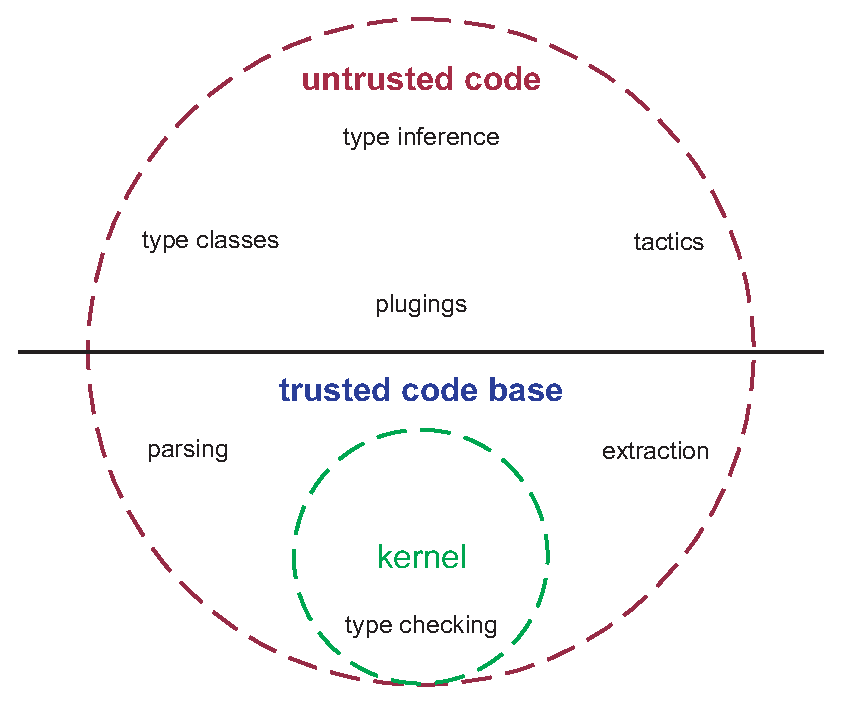
\includegraphics[width=8cm]{pictures/circ.eps}
    \vfill
    {\hfill\cite{SozeauPic}}
\end{frame}


\begin{frame}{Questions?}

Examples from this presentation: \\ {\small\url{https://github.com/digamma-ai/formal-verification-intro}}

\vspace*{2\baselineskip}

Contact: 
\begin{itemize}
    \item Vadim Zaliva, 
\includegraphics[height=\fontcharht\font`\B]{email.png}\ \href{mailto:vzaliva@cmu.edu}{vzaliva@cmu.edu}, 
\includegraphics[height=\fontcharht\font`\B]{Twitter_Social_Icon_Square_Color.png}\ \href{https://twitter.com/vzaliva}{@vzaliva}
    \item Nika Pona, 
\includegraphics[height=\fontcharht\font`\B]{email.png}\ \href{mailto:npona@digamma.ai}{npona@digamma.ai}
\end{itemize}




\end{frame}
    
\begin{frame}[allowframebreaks]{References}

  \bibliography{demo}
  \bibliographystyle{apalike}

\end{frame}

\end{document}